% !TEX root = master.tex
\chapter{Anwendung} \label{chapter:3}
%Grafische Darstellung des Lernprozesses, zentraler Ergebnisse und Beispiele der Agenten.

Die in \ref{chapter:2} beschriebenen Methoden erwiesen sich bei ihrer Anwendung auf das \enquote{Soccer Tows} Problem als unterschiedliche erfolgreich.

\iffalse %temporär auskommentiert

%Single Agent Methods

\ref{fig:bild} zeigt den Belohnungswert der verschiedenen Algorithmen.

Vergleich der verschiedenen Methoden mit Werten für die angepassten Belohnungsstruktur links und original Belohung (Tor oder Gegentor) für ein Spiel rechts.
\begin{figure}[h]
	\centering
	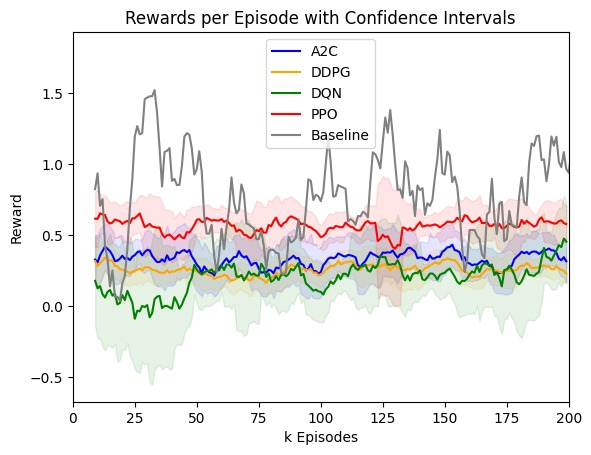
\includegraphics[width=\textwidth]{img/example1.jpeg}
	\caption{Caption}
	\label{fig:bild}
\end{figure}

Es ist zu erkennen



\ref{fig:bild2} zeigt ein Vergleich der verschiedenen Methoden mit Werten für die angepassten Belohnungsstruktur links und original Belohung (Tor oder Gegentor) für ein Spiel rechts.
\ref{fig:bild2} stellt .... dar. 

\begin{figure}[h]
	\centering
	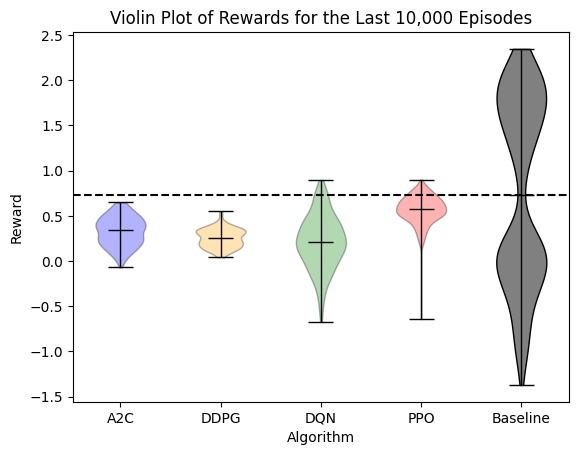
\includegraphics[width=\textwidth]{img/example2.jpeg}
	\caption{Caption ANDERE GRAFIK}
	\label{fig:bild2}
\end{figure}
Es ist zu erkennen, dass die Off-Policy Methoden \ac{XY} und \ac{XY} die schlechtesten Ergenisse liefern. \ac{XY} zeigt einen mit ... einen mitterleren Erfolg. Die besten Ergenisse erziehlt der \ac{PPO} Algorithmus, welcher ... .
Im Vergleich zu der entwickleten Baseline-Methode ist es ersichtlich das .... .


Auch diese Darstellung unterstricht die zuvor beschriebenen Erkennisse. (... was hier noch neu rausgelsen wird)


%MARL

Die Anweung des \enquote{competetiv-self play} Verfahrens für das Mulit-Agent-Szenario ....

\fi



%single agent vergleich
%line chart ppo am besten kein super lernverlauf
%whisker